\documentclass[helvetica]{seminar} 
\input{xy}
\xyoption{all}

\usepackage{graphicx} 
\usepackage{slidesec} 
\usepackage{url} 
\usepackage{amsmath}
\usepackage{amsfonts}
\usepackage[usenames]{color}

\UseCrayolaColors

\long\def\symbolfootnote[#1]#2{\begingroup%
\def\thefootnote{\fnsymbol{footnote}}\footnote[#1]{#2}\endgroup}

% to fix problems making landscape seminar pdfs
% Letter...
\pdfpagewidth=11truein
\pdfpageheight=8.5truein
\pdfhorigin=1truein     % default value(?), but doesn't work without
\pdfvorigin=1truein     % default value(?), but doesn't work without
% A4
%\pdfpagewidth=297truemm % your milage may vary....
%\pdfpageheight=210truemm
%\pdfhorigin=1truein     % default value(?), but doesn't work without
%\pdfvorigin=1truein     % default value(?), but doesn't work without



\renewcommand{\familydefault}{\sfdefault}  
 
\input{seminar.bug} 
\input{seminar.bg2} % See the Seminar bugs list 
 
\slideframe{none} 
 
 
\usepackage{fancyhdr} 
 
% Headings and footers personalization using the `fancyhdr' package 
\fancyhf{} % Clear all fields 
\renewcommand{\headrulewidth}{0mm} 
\renewcommand{\footrulewidth}{0.1mm} 
 
\fancyfoot[L]{\tiny IETF 83} 
\fancyfoot[C]{\tiny Eric Rescorla}
\fancyfoot[R]{\tiny \theslide} 
 
 
% To center horizontally the headings and footers (see seminar.bug) 
\renewcommand{\headwidth}{\textwidth} 

% To adjust the frame length to the heading and footer ones 
\autoslidemarginstrue 
\pagestyle{fancy} 
 

\newcommand{\heading}[1]{% 
  \begin{center} 
    \large\bf 
    #1 
  \end{center} 
  \vspace{.4 in}} 

\begin{document}
\begin{slide}
\begin{center}
\vspace{1 in}
\LARGE{Patching Security Protocols is Hard:\\Lessons from the TLS Experience}
\vspace{.25in}
\large{Eric Rescorla}\\
\url{ekr@rtfm.com}\\
\vspace{.5in}
\large{{IETF 83}} \\
\vspace{.45in}
\end{center}
\end{slide}


% don't center vertically
\centerslidesfalse 


\begin{slide}
\heading{Review: The SSL/TLS Handshake}

\vspace{-.2in} 
\xy
\xymatrix"*"@C=3in@R=.37in{
  \txt{\textbf{Client}} & \txt{\textbf{Server}} \\
  \ar[r]^{\txt{ClientHello}} & \\
  & \ar[l]_{\txt{ServerHello, Certificate}}^{\txt{ServerKeyExchange*, ServerHelloDone}} \\
  \ar[r]^{\txt{ClientKeyExchange, ChangeCipherSpec}}_{\txt{\textsl{Finished}}} & \\
  & \ar[l]_{\txt{ChangeCipherSpec}}^{\txt{\textsl{Finished}}} \\
  \ar@{<->}[r]^{\txt{\textsl{Encrypted traffic}}} & \\
}

\POS(70,5)
\xymatrix{
\txt{Version, Available Ciphers}  \ar(45,-8)
}
\POS*\frm{-}


\POS(0,-15)
\xymatrix{
\txt{Version, Selected Cipher}  \ar(35,-20)
}
\POS*\frm{-}

\POS(70,-15)
\xymatrix{
\txt{RSA Key}  \ar(53,-20)
}
\POS*\frm{-}


\POS(0,-40)
\xymatrix{
\txt{Encrypted Random Value}  \ar(35,-35)
}
\POS*\frm{-}


\POS(75,-40)
\xymatrix{
\txt{Handshake MAC} \ar(52,-38) \ar(52,-48)
}
\POS*\frm{-}
\endxy
\end{slide}

\begin{slide}
\heading{SSL/TLS Negotiation Mechanisms}

\begin{itemize}
\item Version number
\item Cipher suites
\item ``certificate types'' field in \textsf{CertificateRequest}
\item Extensions (published in 2003)~\cite{rfc3546}
\end{itemize}
\end{slide}


\begin{slide}
\heading{}

\end{slide}



\begin{slide}
\heading{Cipher Block Chaining Issues}

\begin{itemize}
\item SSL/TLS, IPsec, and S/MIME all designed around CBC
\item SSL/TLS is especially bad here 
  \begin{itemize}
  \item Implicit (inter-packet) IV until TLS 1.1
  \item Authenticate then Encrypt (AtE), not Encrypt then Authenticate (EtA)~\cite{krawczyk-encryption-order}
  \end{itemize}
  
\item Several known attacks on CBC as used in SSL/TLS
  \begin{itemize}
  \item Attacks on the padding~\cite{vaudenay-tls-cbc}
    \begin{itemize}
    \item Fixed with countermeasures
    \end{itemize}

\item Attacks based on predictable IVs~\cite{moeller-tls-cbc}
    \begin{itemize}
    \item Clumsy countermeasures
    \item Repaired in TLS 1.1~\cite{rfc4346} and DTLS~\cite{modadugu-rescorla:dtls:ndss2004}
    \end{itemize}
\end{itemize}
  \end{itemize}

\end{slide}



\begin{slide}
\heading{CBC Padding Reminder (SSL/TLS variant)}

\begin{center}
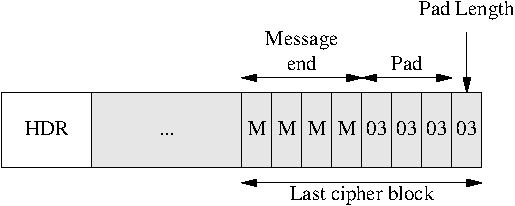
\includegraphics[width=3in]{cbc-pad}

\end{center}
\end{slide}



\begin{slide}
\heading{CBC Attack~\cite{vaudenay-tls-cbc}}

\begin{itemize}
\item Capture cipher block pair $C_i, C_{i+1}$
  \begin{itemize}
  \item Our target is block $C_{i+1}$
  \item Specifically the last byte of block $C_{i+1}$
  \end{itemize}

\item To test our guess for the last byte $==X$, we generate a record ending in
  \begin{itemize}
  \item $C_i \oplus X, C_{i+1}$
  \end{itemize}

\item If we are right, we end up with the last byte == 0 (no padding)
  \begin{itemize}
  \item The MAC check now fails
  \item But SSL/TLS has a different error message for padding and MAC errors
  \item And there is a timing analysis variant
  \end{itemize}
\end{itemize}
\end{slide}


\begin{slide}
\heading{Defenses to CBC attack}

\begin{itemize}
\item ``Right'' approach is to go to EtA
  \begin{itemize}
  \item This blocks record tampering attacks
  \end{itemize}

\item Instead SSL/TLS uses a bunch of countermeasures
  \begin{itemize}
  \item Return \textsl{mac\_error} for all decoding errors
  \item Bogus MAC check to hide timing channel
  \end{itemize}

\item Why?
  \begin{itemize}
  \item Attack is very inefficient
    \begin{itemize}
    \item SSL/TLS terminates after decoding errors (but DTLS...)
    \end{itemize}
  \item Unilateral versus bilateral changes
  \end{itemize}
\end{itemize}

\end{slide}



\begin{slide}
\heading{Review of Predictable IV attacks}

\begin{itemize}

\item Scenario: Attacker can observe ciphertext and inject his own plaintext
  \begin{itemize}
  \item He observes a block $C_i$ and wants to verify his guess $X$ for its value
  \end{itemize}

\item Attacker sees a record with trailing block $B$
  \begin{itemize}
  \item This means that $B$ is the IV for the next block
  \end{itemize}

\item Attacker injects $C_{i-1} \oplus B \oplus X$ as plaintext
  \begin{itemize}
  \item Victim encrypts $B \oplus C_{i-1} \oplus B \oplus X = C_{i-1} \oplus X$
  \item If result is $C_i$ then the guess was correct
  \end{itemize}
\end{itemize}

\end{slide}



\begin{slide}
\heading{Limitations of Predictable IV Attacks}

\begin{itemize}
\item Need tight control of the channel
  \begin{itemize}
  \item Didn't seem likely except for VPN settings
  \end{itemize}

\item Need to guess an entire block at a time
  \begin{itemize}
  \item Not easy!
  \end{itemize}

\item This all doesn't sound very serious
  \begin{itemize}
  \item TLS WG duly fixed TLS~\cite{rfc4346}
  \item But practically nobody implemented it
  \end{itemize}
\end{itemize}

\end{slide}






\begin{slide}
\heading{Predictions are hard... especially about the future}

\vspace{-.25in}
\begin{itemize}
\item Rizzo/Duong ``BEAST'' paper changed people's perceptions of the risk
  \begin{itemize}
  \item New technique for byte-by-byte guessing
  \item New threat vector via Web technologies (WebSockets and Java)
  \end{itemize}

\item But this was fixed in TLS 1.1
  \begin{itemize}
  \item So we'll just deploy TLS 1.1, right?
  \item Well sort of...
  \end{itemize}

\item People are deploying TLS 1.1
  \begin{itemize}
  \item But \emph{also} 1/n+1 splitting countermeasure
  \item And active attacks on TLS version negotiation are possible
  \end{itemize}

\end{itemize}
\end{slide}


\begin{slide}
\heading{Implementing for extensibility is really hard}

\vspace{-.25in}

\begin{scriptsize}
\begin{quote}
   ``Note: some server implementations are known to implement version
   negotiation incorrectly.  For example, there are buggy TLS 1.0
   servers that simply close the connection when the client offers a
   version newer than TLS 1.0.  Also, it is known that some servers will
   refuse the connection if any TLS extensions are included in
   ClientHello.  Interoperability with such buggy servers is a complex
   topic beyond the scope of this document, and may require \emph{multiple
   connection attempts by the client.}\symbolfootnote[1]{emphasis mine}

   Earlier versions of the TLS specification were not fully clear on
   what the record layer version number (TLSPlaintext.version) should
   contain when sending ClientHello (i.e., before it is known which
   version of the protocol will be employed).  Thus, TLS servers
   compliant with this specification MUST accept any value {03,XX} as
   the record layer version number for ClientHello.

   TLS clients that wish to negotiate with older servers MAY send any
   value {03,XX} as the record layer version number.  Typical values
   would be {03,00}, the lowest version number supported by the client,
   and the value of ClientHello.client\_version.  No single value will
   guarantee interoperability with all old servers, but this is a
   complex topic beyond the scope of this document.''~\cite{rfc5246}
\end{quote}
\end{scriptsize}

\end{slide}

\begin{slide}
\heading{A simple downgrade attack}

\vspace{-.2in} 
\xy
\xymatrix"*"@C=1in@R=.25in{
  \txt{\textbf{Client}} & \txt{\textbf{Attacker}} & \txt{\textbf{Server}} \\
  \ar[r]^{\txt{ClientHello (version 1.1)}} & \\
  & \ar[l]_{\txt{TCP RST}} \\
  \txt{[Client falls back]} \\
  \ar[rr]^{\txt{ClientHello (version 1.0)}} & &\\
  & \txt{...} & \\
}
\endxy

\begin{itemize}
\item Attacker pretends to be a broken server
\item This bypasses all TLS anti-downgrade mechanisms
\end{itemize}

\end{slide}








\begin{slide}
\heading{Questions?}

\end{slide}





\begin{slide}
\footnotesize{
\bibliographystyle{alpha}
\bibliography{rfc,rescorlabib,ekr-it}
}
\end{slide}


\end{document}